\begin{figure}
  \centering
  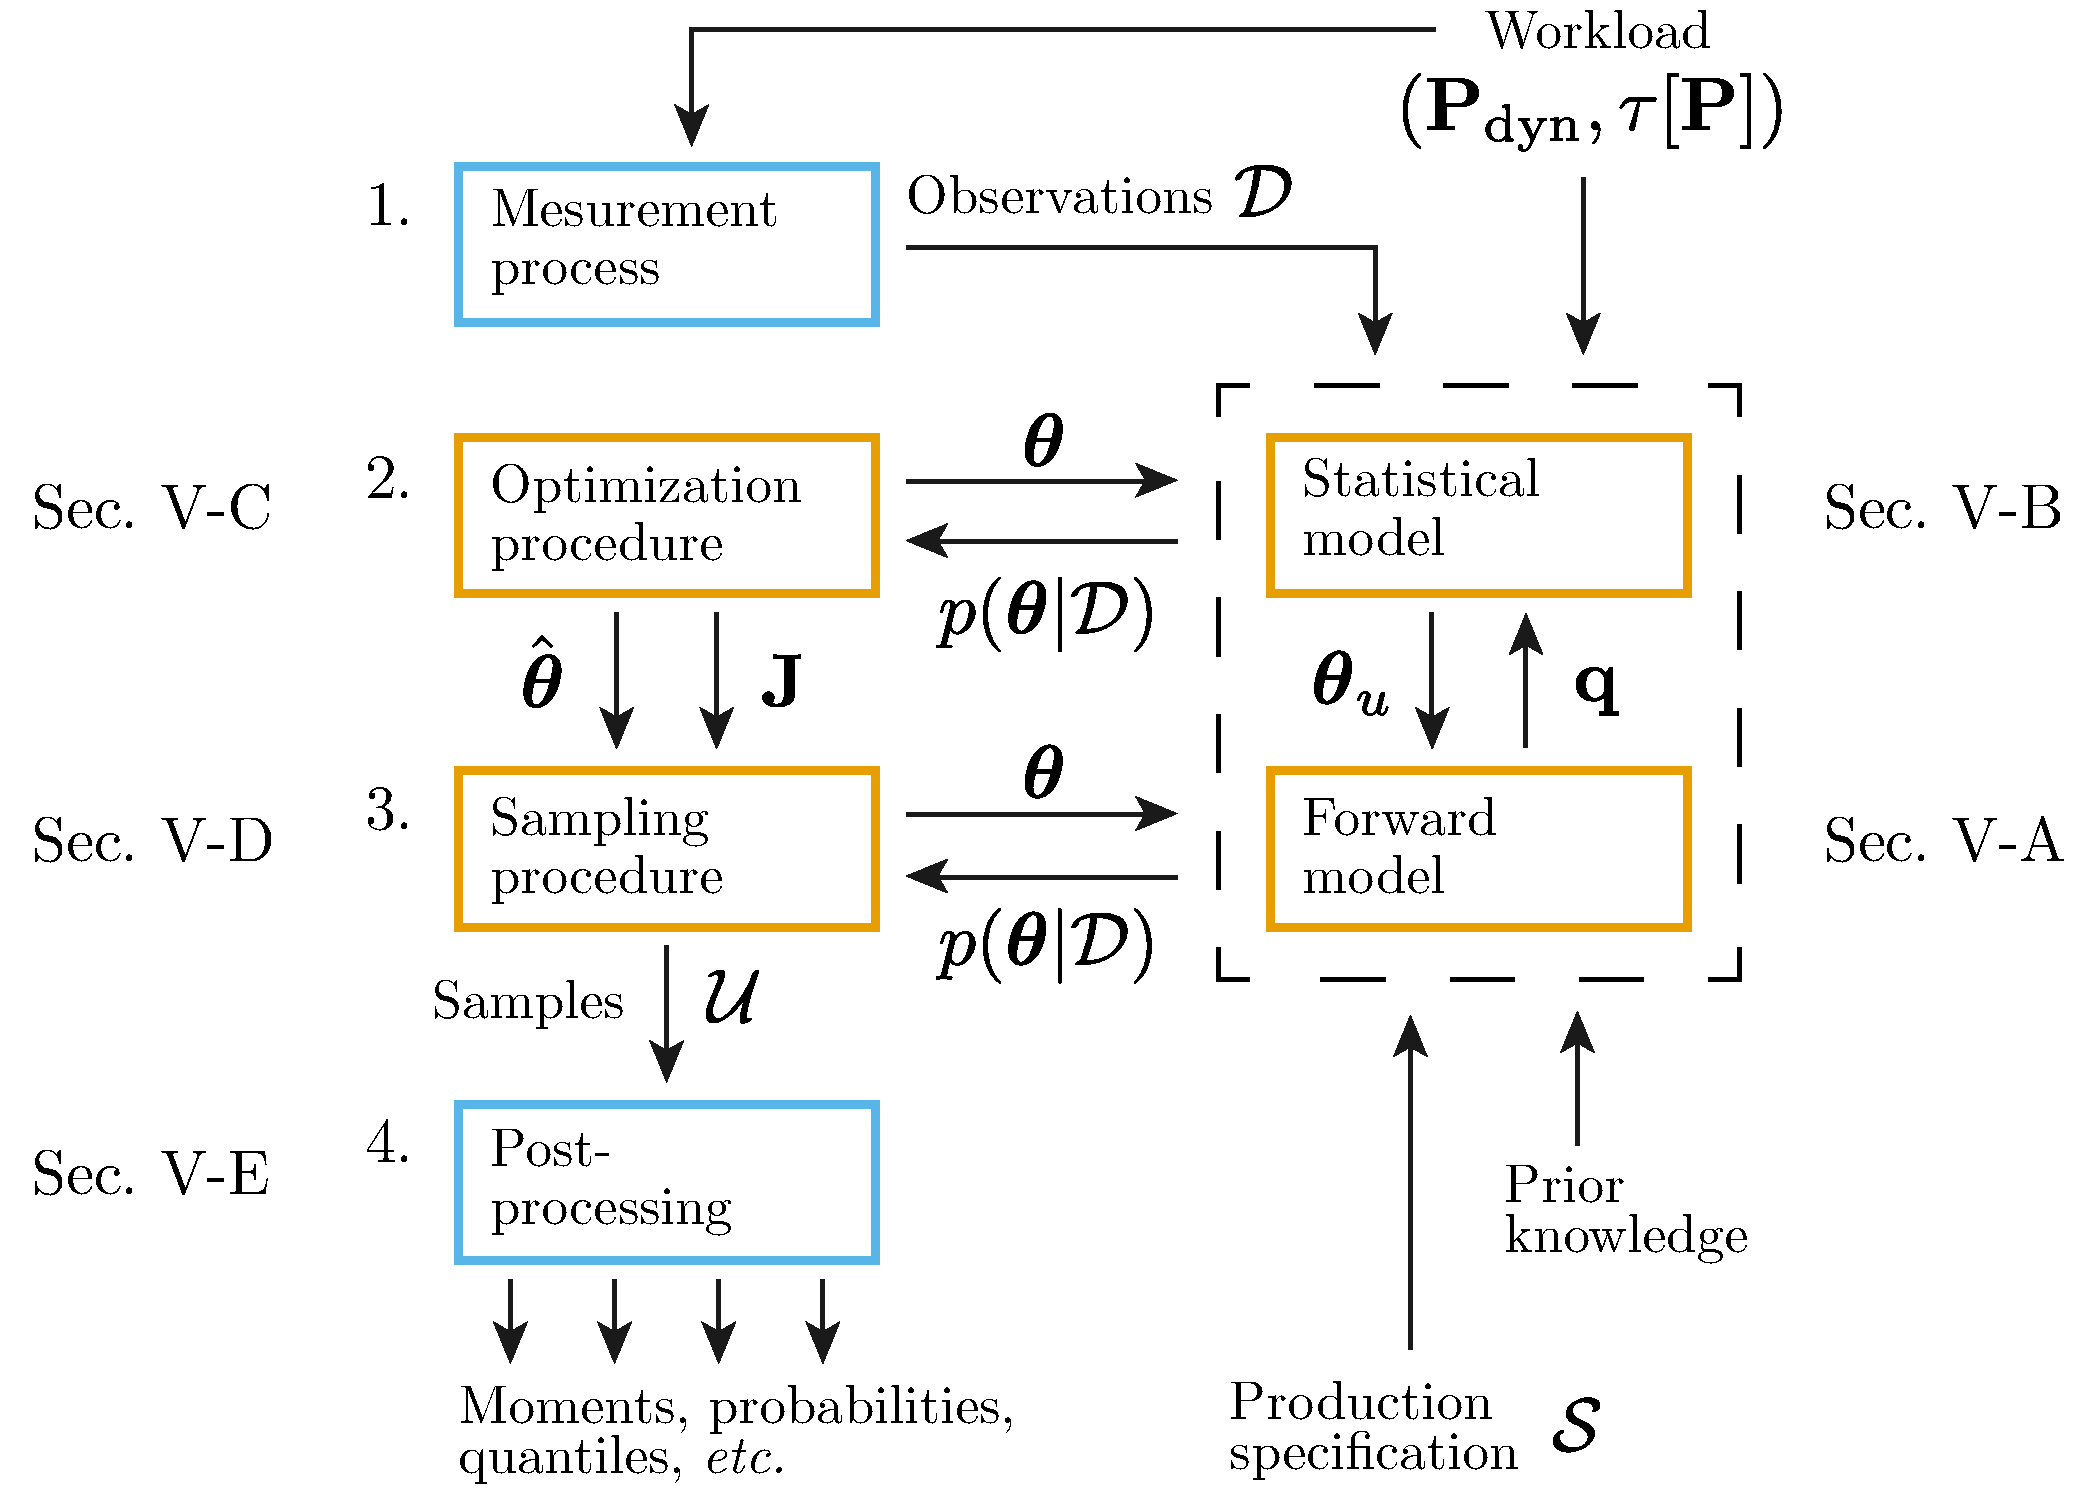
\includegraphics[width=0.80\linewidth]{include/figures/algorithm.pdf}
  \caption{The proposed framework.}
  \flabel{algorithm}
\end{figure}

In this section, we present our statistical framework for the characterization of process variation.
The technique is divided into four major stages depicted in \fref{algorithm}.
\stage{1}\ is the data-harvesting stage wherein the user collects a set of observations of the \qom, $\q$, forming $\QData$.
At \stage{2}, we undertake an optimization procedure, which assists the MCMC sampling at \stage{3}\ in the construction of an efficient proposal distribution.
\stage{3}\ produces a collection of samples of the \qoi, $\u$, such as the effective channel length, which is then processed at \stage{4}\ in order to estimate all the needed characteristics of this \qoi, \eg, the probability of the effective channel length to be smaller than a certain threshold as motivated in \sref{motivation}.
As it can be seen in \fref{algorithm}, \stage{2}\ and \stage{3}\ actively communicate with two models on the right, called the data and statistical models, which we shall discuss next.

\subsection{Data Model} \slabel{data-model}
The data model is essentially a directed relation between the \qoi, $\u$, and the \qom, $\q$, which we denote by the ``black-box'' transformation $\q = \oBB{\u}$.
$\oBB$ depends on the choice of $\q$ and is specified by the user according to the guidelines in \sref{problem-formulation}.

In order to acquire a better understanding of the data model, let us return to the setup considered in \sref{motivation}.
In this case, $\u$ stands for the effective channel length, and $\q$ stands for the temperature profile corresponding to a fixed workload given as, \eg, a dynamic power profile.
The choice of $\u$ and $\q$ for illustration is dictated by the fact that such a high-level parameter as temperature constitutes a challenging task for the inference of such a low-level parameter as the effective channel length, which implies an intense assessment of the propose technique.
The performance of our framework is expected to increase when the auxiliary parameter $\q$ that resides ``closer'' to the target parameter $\u$ with respect to the transformation $\q = \oBB{\u}$ provided that the amount and granularity of the measurement data stay the same.
For example, such a ``closer'' quantity $\q$ can be the leakage current; however, the leakage current is not always the most preferable parameter to work with.

In the ongoing example, the data model $\q = \oBB{\u}$ can be roughly divided into two transitions: (a) the effective channel length $\u$ to the leakage power $\p_\leak$ and (b) the leakage power $\p_\leak$ to the corresponding temperature profile $\q$.
The first transition is accomplished using one of the leakage models broadly found in the contemporary literature; see, \eg, \cite{chandrakasan2001, srivastava2010, juan2012}.
In particular, a leakage model can be constructed via a fitting procedure applied a data set of SPICE simulations of reference electrical circuits.
The only requirement to such a model is that it should be parametrized by $\u$.
In addition, it can also be parametrized by temperature in order to account for the well-known interdependency between leakage and temperature.
The second transition is undertaken by combining the leakage power $\p_\leak$ with the dynamic power $\p_\dyn$ that corresponds to the considered workload used for heating the dies.
The obtained total power along with the temperature-related information contained in $\specification$ (mainly, the floorplan and thermal parameters of the die) are fed to a thermal simulator in order to acquire the corresponding temperature $\q$.

Without loss of generality, in the experimental results reported in \sref{experimental-results}, we use a temperature-aware model for leakage attained via fitting to SPICE simulations, and the temperature calculations are undertaken in the same way as the one described in \cite{ukhov2012}, which is based on the HotSpot thermal model \cite{hotspot}.


\subsection{Statistical Model} \slabel{statistical-model}
Since, at each point of the continuum of spatial locations on the wafer, $\U$ can potentially take a different value, $\U$ is infinite-dimensional. We model $\U$ as a square-integrable stochastic process $\U: \omega \times \domain \to \real$ defined over a spacial domain $\domain$ corresponding to the wafer. Denote the forward model developed in \sref{power-model} and \sref{thermal-model} by
\begin{equation} \elabel{model}
  \mT(\r) = \model{\mP_\dyn, \r | \u}
\end{equation}
which, for an outcome $\u: \domain \to \real$ of the process $\U$, transforms an arbitrary dynamic power profile $\profilePdyn$ into the corresponding temperature profile $\profileT$ computed at location $\r \in \domain$. Note, $\model$ also performs thinning of the output temperature to match the partition $\partition{\mT}$ of $\data$. Since $\U(\r)$ is a random element, so $\mT(\r)$ is. Moreover, even if $\U(\r)$ was given (fixed), due to the imperfection of the modeling and measurement processes, a temperature profile $\mT^{(i)}_\meas$ from the data set $\data$ is assumed to deviate from the model prediction in \eref{model}. To account for this, $\mT^{(i)}_\meas$ is modeled as
\[
  \mT^{(i)}_\meas = \mT(\r_i) + \mnoise^{(i)} = \model{\mP_\dyn, \r_i | \u} + \mnoise^{(i)}
\]
where $\mnoise^{(i)} = (\noise^{(i)}_{jk}) \in \real^{\ncores \times \nsteps}$ represents a matrix of an additive noise. Such a noise is typically assumed to be a white Gaussian noise and to be independent from the parametrization $\U(\r)$ \cite{marzouk2007, el-moselhy2012}. Therefore, $\noise^{(i)}_{jk}$ is modeled as
\[
  \noise^{(i)}_{jk} \sim \gaussian{0}{\sigma^2_\noise}
\]
where, imposing no loss of generality, the noise is assumed to have the same magnitude for all measurements. Now, we can form the likelihood function $\f{\data | \u}$ of the data $\data$, which, intuitively speaking, gives the probability of observing $\data$:
\begin{align}
  \f{\data | \u} & = \prod_{i = 1}^{\ndata} \f{\mT^{(i)}_\meas, \r_i | \u} \nonumber \\
  & = \left(2 \pi \sigma_\noise^2\right)^{-\frac{\ndcs}{2}} \exp\left( -\frac{1}{2 \sigma^2_\noise} \sum_{i = 1}^\ndata \fnorm{\mnoise^{(i)}}^2 \right) \elabel{likelihood}
\end{align}
where $\ndcs = \ndata \ncores \nsteps$, $\fnorm{\cdot}$ is the Frobenius norm, and
\[
  \mnoise^{(i)} = \mT^{(i)}_{\meas} - \mT(\r_i) = \mT^{(i)}_{\meas} - \model{\mP_\dyn, \r_i | \u}.
\]
The likelihood function in \eref{likelihood} corresponds to the density of a Gaussian vector with $\ndcs$ independent components:
\[
  \data | \u \sim \gaussian{\vectorize{\model{\mP_\dyn, \vr | \u}}}{\sigma_\noise^2 \mI_\ndcs}
\]
where $\vectorize{\cdot}$ stands for the vectorization of a matrix or a set of matrices, \ie, columns of matrices are successively stacked into a single vector. In the notation above, the left-hand side is a shortcut for $\vectorize{\{ \mT_\meas^{(i)} \}_{i = 1}^\ndata} | \u$, and the right-hand side means that the forward model $\model$ is to be evaluated for each $\r_i$ in $\vr$, and the resulting matrices are then vectorized.

Now, we need to identify the stochastic process $\U(\r)$ in order to specify the prior, which the density $\f{\u}$ in \eref{bayes} corresponds to. Uncertainties due to process variation are known to be well approximated using Gaussian distributions \cite{srivastava2010}; therefore, $\U(\r)$ is assumed to be a Gaussian process \cite{rasmussen2006}:
\[
  \U(\r) \sim \gaussian{\fMean{\r}}{\fCov{\r, \r'}}
\]
where $\fMean{\r} := \E{\U(\r)}$ and $\fCov{\r, \r'}$ are the expectation and covariance functions of $\U(\r)$. Due to the particularities of the manufacturing process, such uncertainties often bear radial structures \cite{cheng2011}; thus, we assume that $\r$ represents the Euclidean distance from the center of the wafer to the center of the die, and the covariance function of $\U(\r)$ belongs to the squared exponential family of covariance functions \cite{rasmussen2006}:
\begin{equation} \elabel{covariance-function}
  \fCov{\r, \r'} = \sigma^2_\U \exp\left(-\frac{1}{2 \ell}(\r - \r')^2\right)
\end{equation}
where $\sigma^2_\U$ stands for variance, and $\ell > 0$ is the correlation length. Now, let $\vr^* = (\r^*_i) \in \real^n$ be a vector of spatial locations of interest. Then the prior over these locations is
\begin{equation} \elabel{prior}
  \f{\u | \vr^*} = \left(|2 \pi \mCov|\right)^{-\frac{1}{2}} \exp\left(-\frac{1}{2} (\vu - \vfMean)^T \mCov^{-1} (\vu - \vfMean) \right)
\end{equation}
where $\vu = \u(\vr^*) := (u(\r^*_i)) \in \real^n$, $\vfMean = \fMean{\vr^*} := (\fMean{\r^*_i}) \in \real^n$, $\mCov = (\fCov{\r^*_i, \r^*_j}) \in \real^{n \times n}$, and $|\cdot|$, applied to a matrix, denotes the matrix determinant. Equivalently,
\[
  \u | \vr^* \sim \gaussian{\vfMean}{\mCov}
\]
where $\u | \vr^*$ stands for $\u(\vr^*)$.

Due to the forward model $\model$ involved in \eref{likelihood}, there is no convenient expression for the posterior density $\f{\u | \data}$ in \eref{bayes}. As mentioned in \sref{bayesian-inference}, to overcome the difficulty, we utilize the Metropolis-Hastings algorithm \cite{gelman2004}. To this end, we combine \eref{likelihood} with \eref{prior} and compute, up to a constant summand, the logarithm of the posterior:
\begin{align*}
  & \log \f{\u | \data, \vr^*} = \log \f{\data | \u} + \log \f{\u | \vr} + c_1 \\
  & = -\frac{1}{2 \sigma^2_\noise} \sum_{i = 1}^\ndata \fnorm{\mnoise^{(i)}}^2 -\frac{1}{2} (\vu - \vfMean)^T \mCov^{-1} (\vu - \vfMean) + c_2 \\
  & = - A(\u | \data) - B(\u | \vr^*) + c_2
\end{align*}
where $c_1$ and $c_2$ are constants with respect to $\u$, which are irrelevant for our purposes, and
\begin{align*}
  & A(\u | \data ) = \frac{1}{2 \sigma^2_\noise} \sum_{i = 1}^\ndata \fnorm{\mT^{(i)}_{\meas} - \model{\mP_\dyn, \r_i | \u}}^2, \\
  & B(\u | \vr^*) = \frac{1}{2} (\vu - \vfMean)^T \mCov^{-1} (\vu - \vfMean).
\end{align*}
It is worth being noted that $A(\u | \data)$ poses a significant computational challenge as it requires $\ndata$ evaluations of $\model$ for each sample of $\U$.


\subsection{Optimization of the Proposal Distribution} \slabel{optimization}
In this section, we describe the objective of Stage~2 in \fref{algorithm}.
Although the requirements to the proposal distribution mentioned earlier are rather weak, it is often difficult to pick an efficient proposal, which would yield a good approximation with as fewer evaluations of the posterior in \eref{posterior} and, thus, of the data model in \sref{data-model} as possible.
This choice is especially severe for high-dimensional problems, and our problem, involving around 30 parameters as we shall see in \sref{experimental-results}, is one them.
Therefore, a careful construction of the proposal is an essential component of our framework.
A common technique to construct a high-quality proposal is to perform an optimization procedure of the posterior given by \eref{posterior}.
More specifically, we seek for such a value $\hat{\vparam}$ of $\vparam$ that maximizes \eref{posterior} and, hence, has the maximal posterior probability.
We also compute the negative of the Hessian matrix at $\hat{\vparam}$, which is called the observed information matrix and denoted by $\mOI$ (see the output of Stage~2 in \fref{algorithm}).
Using $\hat{\vparam}$ and $\mOI$, we can now construct such a proposal, which will allow the MH algorithm (a) to start producing samples directly from the desired regions of high probability and (b) to explore those regions more rapidly.


\subsection{Sampling via the Metropolis-Hastings Algorithm} \slabel{sampling}
\slabel{proposal-distribution}
As discussed in \sref{bayesian-inference}, the core of the Metropolis algorithm is the proposal distribution. A carefully constructed proposal can significantly reduce the number of steps needed for the corresponding Markov chain to start producing representative samples; in other words, it can save a lot of forward model evaluations.
A common technique to construct a high-quality proposal is to undertake an optimization procedure of the log-posterior given by \eref{log-posterior}, which we also do. Specifically, we seek for such a value of $\vparam$ that maximizes \eref{log-posterior}.
Consequently, the optimization yields a highly probable value of $\vparam$, denoted by $\hat{\vparam}$, along with the corresponding Hessian matrix, denoted by $\mOI$. The two form a solid base for the proposal.
For example, a classical choice of such a distribution is a multivariate Gaussian distribution wherein the mean is the current location of the Markov chain started from $\hat{\vparam}$, and the covariance matrix is the inverse of $\mOI$; see \cite{gelman2004, bernardo2007}.

\slabel{sampling-strategy}
In order to speed up the inference process even further, we make use of the omnipresent multicore parallelization for sampling. To this end, instead of utilizing the classical proposal mentioned in the previous paragraph---which is purely sequential as the mean for the next sample draw is dependent on the previous sample---we appeal to the independence sampler Metropolis algorithm \cite{gelman2004}. In this case, a typical choice of the proposal is a multivariate t-distribution, which is independent of the current position of the chain:
\begin{equation} \elabel{proposal}
  \vparam \sim \studentst{\nu}{\hat{\vparam}}{\alpha^2 \mOI^{-1}}
\end{equation}
where $\hat{\vparam}$ and $\mOI$ are as in \sref{proposal-distribution}, $\nu$ is the number of degrees of freedom, and $\alpha$ is a tuning constant. Now, the posterior in \eref{log-posterior} can be computed for all samples in parallel.

Having completed the sampling procedure, we obtain a collection of samples of the parametrization $\vparam$. Since it can take time for a Markov chain to reach regions of high probability (see \sref{bayesian-inference}), a certain number of initial samples are typically discarded as being unrepresentative, which is known as a burn-in period.
Each of the preserved samples of $\vparam$ is then used in \eref{kl-approximation} to compute a sample of $\u$, $\u_i \in \real^{\ndies \nprocs \nsteps}$.
Denote such a data set with $\nsamples$ samples by $\UData = \{ \u_i \}_{i = 1}^\nsamples$.


\subsection{Post-processing} \slabel{post-processing}
At \stage{4}\ in \fref{algorithm}, using the set of samples $\UData$, the user computes the desired statistics of the \qoi\ such as the most probable value of the effective channel length at some location of interest, the probability of a certain area on the wafer to be defective, \etc\ The computations boil down to the estimation of expected values with respect to the posterior distribution of $\vparam$, $\f{\vparam | \QData}$.
This estimation is done in the standard sample-based fashion, that is, in order to compute some arbitrary quantity dependent on $\u$, one needs to evaluate this quantity for each $\vu_i$ in $\UData$ and then take the average.

The strength of the Bayesian approach to inference really starts to shine when we are also interested in assessing the trustworthiness of the measured data and, therefore, the reliability of the estimates/decisions based on these data.
Such an assessment can readily be undertaken using our framework since the delivered posterior distribution contains all the needed information about the \qoi.
This is especially helpful in decision making as exemplified in \sref{motivation}.

